\chapter{Analisi del contesto tecnologico}
\label{cap:analisi-soluzioni-esistenti}

\par Uno dei passi fondamentali nel processo di ottimizzazione SEO è la scelta delle parole chiave e il loro utilizzo in punti strategici delle pagine web. Esistono software in grado di automatizzare la ricerca e l’analisi delle keywords, contribuendo a migliorare il posizionamento e l’indicizzazione del sito. Questi strumenti, disponibili gratuitamente o a pagamento, coprono numerosi aspetti dell’analisi SEO, tra cui:
\begin{itemize}
    \item Analisi SEO on-page (meta tag, intestazioni, URL, immagini, broken link, redirect, ecc.);
    \item Ricerca delle parole chiave per cui un sito web è posizionato in alto nella SERP (Search Engine Results Page);
    \item Suggerimento di parole chiave correlate e rilevanti;
    \item Anteprima SERP per una parola chiave scelta dall'utente;
    \item Analisi dell’efficacia delle parole chiave;
    \item Analisi dei competitor;
    \item Distribuzione delle parole chiave all’interno di una pagina web;
    \item Analisi di parametri essenziali come la keyword difficulty (difficoltà di posizionarsi per una specifica parola chiave) e il keyword stuffing (uso eccessivo di una parola chiave).
\end{itemize}

\section{MozBar}

\subsection{Funzionalità}
\par MozBar è un'estensione gratuita per Chrome che consente agli utenti di eseguire analisi SEO on-page e accedere a metriche avanzate senza aprire un'altra scheda del browser. Le funzionalità fornite dall'estensione includono:
\begin{itemize}
    \item \textbf{Page Authority e Domain Authority}: metriche da 1 a 100 che prevedono il posizionamento di una pagina e un dominio in base a un algoritmo di apprendimento automatico;
    \item \textbf{Linking Domains}: numero di domini unici che puntano a un sito;
    \item \textbf{Inbound Links}: numero di link in entrata provenienti da pagine esterne;
    \item \textbf{Attributi generali}: tempo di caricamento, tag canonical, URL della cache di Google, sitemap, Hreflang, tag robots;
    \item \textbf{Elementi on-page}: URL, titolo, meta description, meta tag keywords, elenco degli heading, testo alternativo delle immagini;
    \item \textbf{Dati strutturati (JSON-LD)}: verifica che lo schema sia formattato correttamente;
    \item \textbf{Ranking Keywords}: identifica le parole chiave per cui un sito è posizionato e fornisce informazioni sui competitor;
    \item \textbf{Ottimizzazione della pagina}: visualizza il punteggio ottenuto per una determinata parola chiave e mostra  i fattori che contribuiscono al punteggio complessivo, nonché quelli che potrebbero danneggiarlo;
    \item \textbf{Highlight links}: evidenzia tutte le tipologie di link presenti all’interno della pagina;
    \item \textbf{Highlight keywords}: questa funzionalità consente agli utenti di inserire una parola chiave e ottenere il numero di occorrenze. Inoltre, la parola chiave viene evidenziata all’interno della pagina.
\end{itemize}

\begin{figure}[H]
    \centering 
    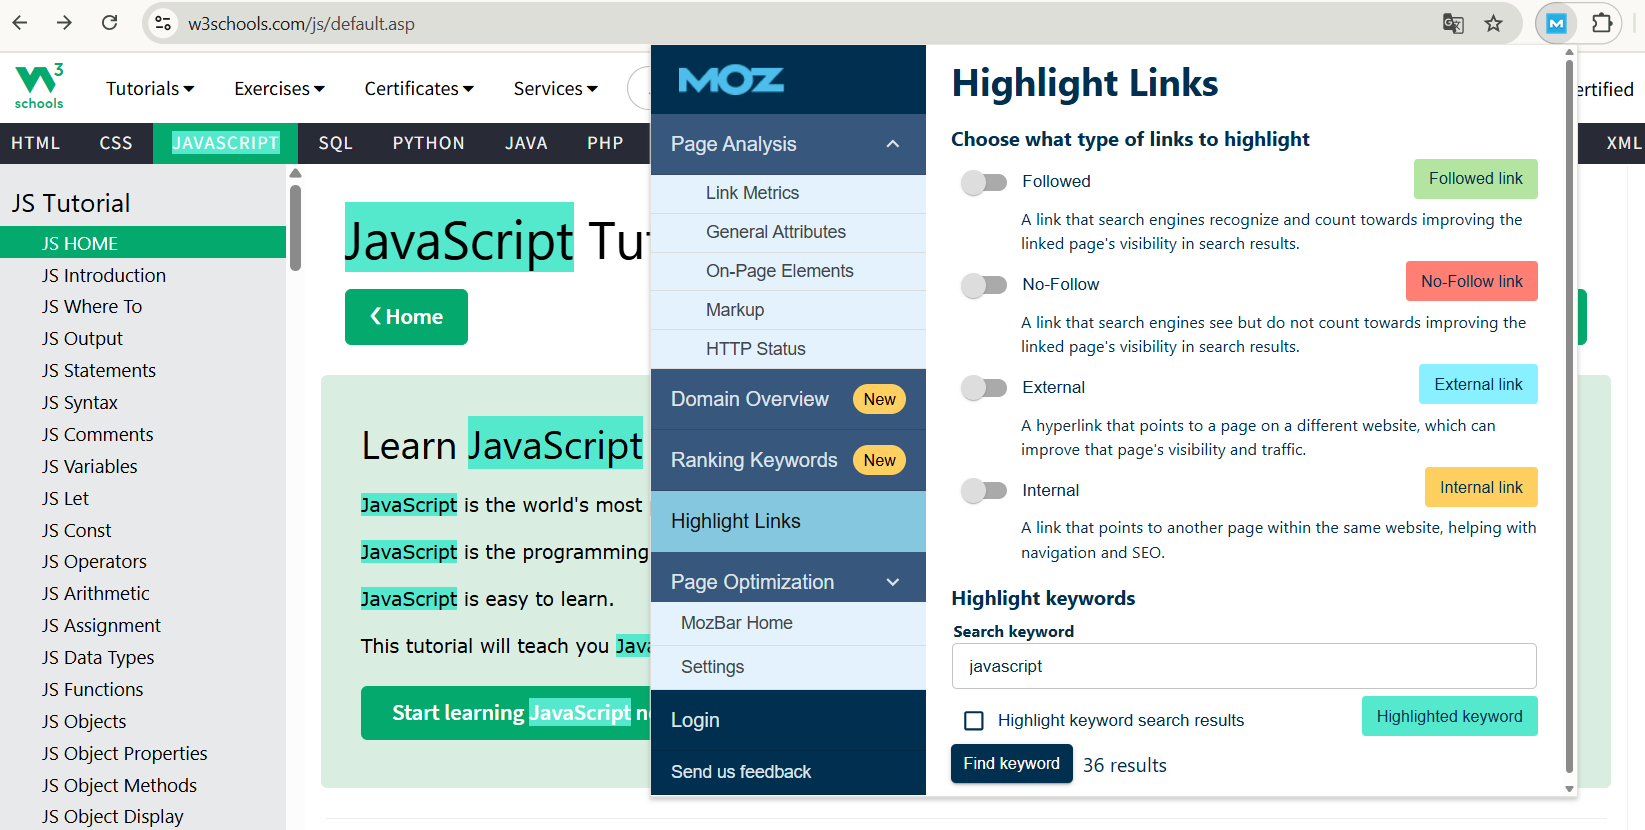
\includegraphics[width=0.8\columnwidth]{soluzioni-esistenti/MozBar/moz_bar_search_keywords.png} 
    \caption{MozBar - Analisi parole chiave}
\end{figure}

\subsection{Vantaggi}
\par Poiché funziona su localhost, l’estensione può essere facilmente usata durante lo sviluppo. La barra degli strumenti può essere ancorata in alto o in basso nella pagina e le metriche SEO possono essere visualizzate direttamente nei risultati di ricerca.

\subsection{Svantaggi}
\par L’estensione non è disponibile come barra laterale, ma solo come pop-up o barra degli strumenti. Inoltre, il rilevamento dei tag è case-sensitive, quindi c’è il rischio che alcuni tag non vengano rilevati se si usa la lettera iniziale maiuscola. La funzionalità di analisi delle parole chiave non include alcuni aspetti, come la densità o la distribuzione. Le funzionalità premium richiedono un abbonamento a pagamento. 

\section{Silktide (analisi SEO su richiesta)}

\subsection{Funzionalità}
\par Le soluzioni progettate da Silktide sono in grado di identificare problemi SEO come titoli mancanti, "broken link", scarsa velocità di caricamento e mancanza di ottimizzazione delle parole chiave. Per quanto riguarda l’analisi delle keywords, Silktide mette a disposizione un modulo di ranking che permette di monitorare:
\begin{itemize}
    \item \textbf{Parole chiave organiche}: portano traffico “organico” (non sponsorizzato) a un sito web. Sono i termini di ricerca per i quali il sito viene posizionato, sulla base di algoritmi di ranking, nella SERP (Search Engine Results Page). Le "SERP previews" mostrano un'anteprima del posizionamento del sito nella pagina dei risultati del motore di ricerca;
    \item \textbf{Parole chiave a pagamento}: portano traffico tramite annunci sponsorizzati. Sono i termini per i quali è stata attivata una campagna pubblicitaria PPC (Pay-Per-Click). "Le PPC previews" mostrano un'anteprima di come appare l'annuncio a pagamento per una determinata keyword.
\end{itemize}
\par Oltre a monitorare le keywords selezionate, Silktide identifica anche i siti che competono per le stesse parole chiave, generando un elenco basato sul numero di keywords in comune.

\begin{figure}[H]
    \centering 
    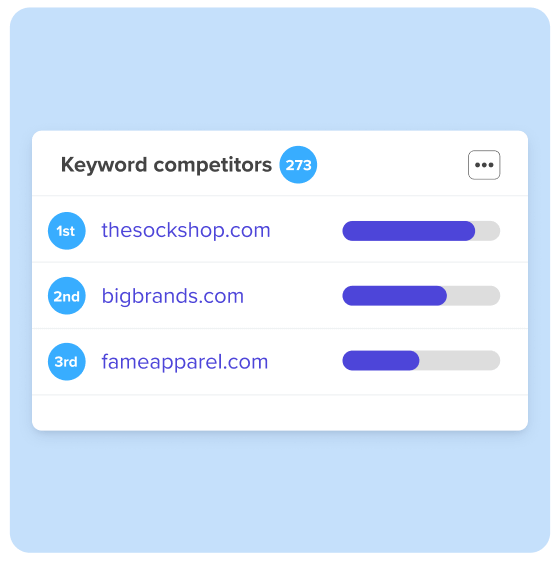
\includegraphics[width=0.6\columnwidth]{soluzioni-esistenti/Silktide/silktide_competitor_analysis.png} 
    \caption{Silktide - Analisi dei competitor}
\end{figure}

\subsection{Vantaggi}
\par Silktide offre funzionalità SEO avanzate come il monitoraggio delle keywords, anteprime SERP e PPC, analisi dei competitor; il tutto integrato in un'unica piattaforma. Il team di Silktide mette a disposizione, su richiesta, una scansione gratuita, personalizzata e interattiva del sito web.

\subsection{Svantaggi}
\par Per usufruire della funzionalità di analisi SEO è necessario prenotare una dimostrazione e attendere l'esito dell'analisi. Si tratta di uno strumento orientato maggiormente a grandi realtà che necessitano di una piattaforma di marketing completa.

\section{Semrush}

\subsection{Funzionalità}
\par Semrush include oltre 50 strumenti di analisi SEO, il che lo rende una delle piattaforme più complete sul mercato. La dashboard consente di visualizzare gratuitamente analisi relative al traffico, ai backlink, alle ricerche organiche e a quelle sponsorizzate. Offre inoltre funzionalità avanzate come:
\begin{itemize}
    \item \textbf{Analisi SEO on-page};
    \item \textbf{Keyword research}: suggerisce parole chiave rilevanti in base al volume di ricerca, all'intento, alla keyword difficulty e ad altri fattori SEO. Questa funzionalità può essere integrato con plugin di terze parti, tra cui Yoast SEO per WordPress;
    \item \textbf{Analisi dei competitor};
    \item \textbf{Position tracking}: monitora il posizionamento nella SERP (Search Engine Results Page) per determinate parole chiave.
\end{itemize}

\begin{figure}[H] 
    \centering 
    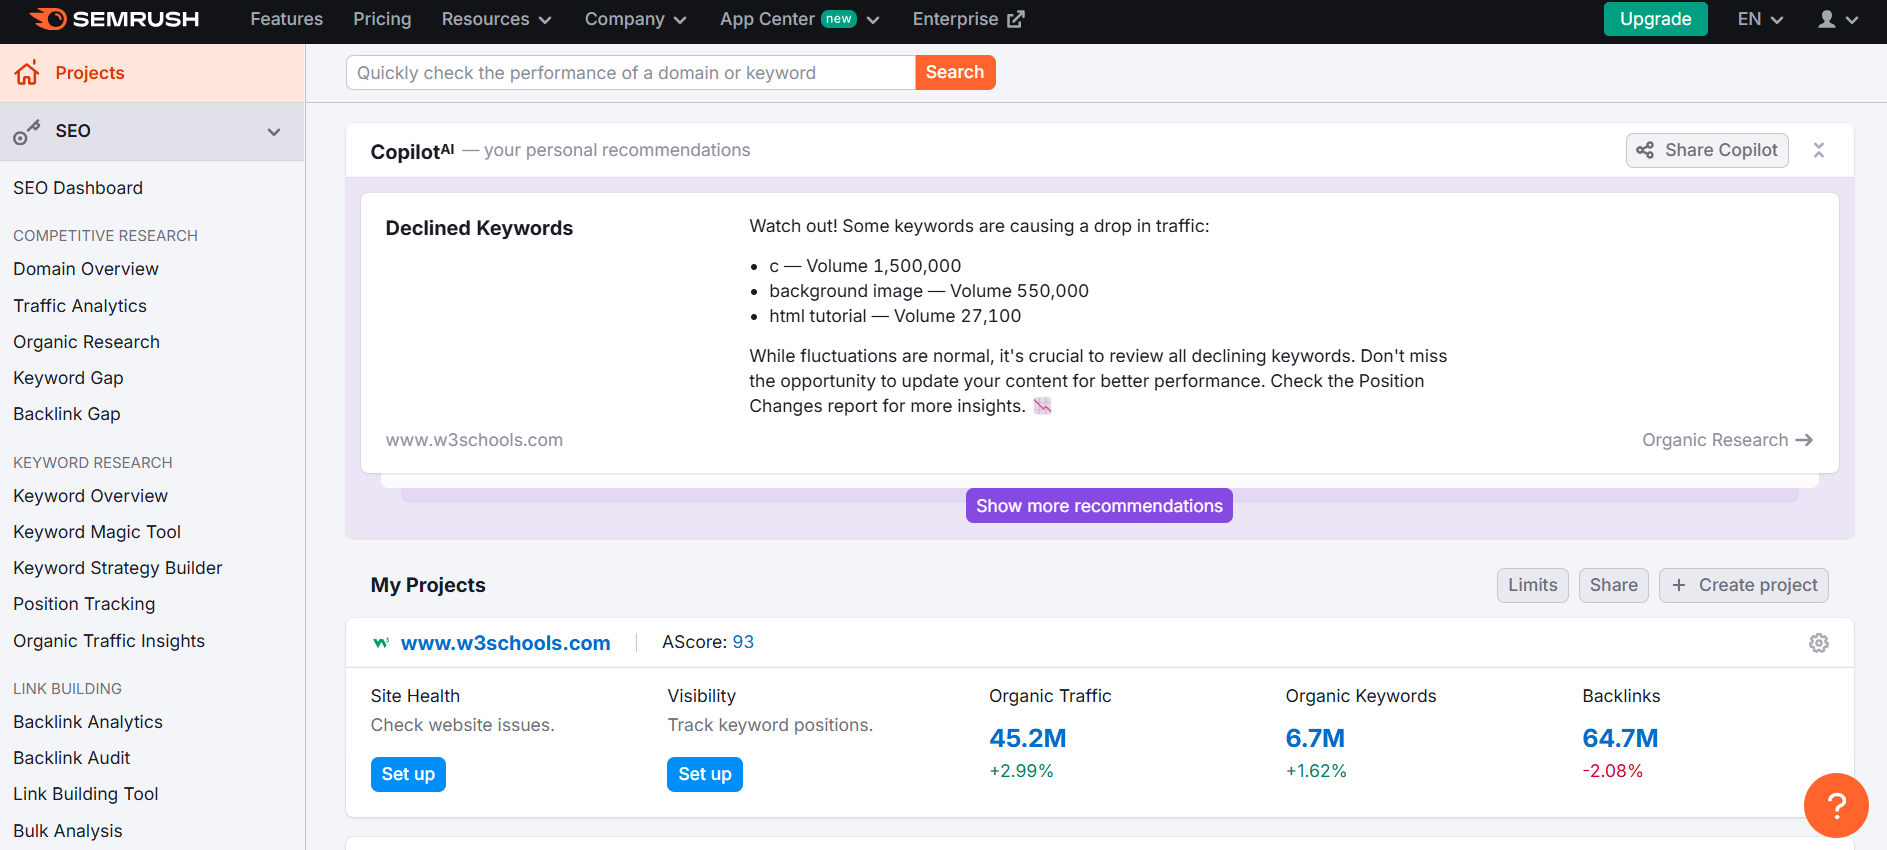
\includegraphics[width=0.9\textwidth]{soluzioni-esistenti/SEMrush/semrush.png} 
    \caption{Semrush - SEO dashboard}
\end{figure}

\subsection{Vantaggi}
\par Semrush può essere integrato facilmente con altri strumenti di analisi SEO. Integra funzionalità tecniche e strumenti di marketing in un'unica piattaforma.

\subsection{Svantaggi}
\par Le funzionalità avanzate sono a pagamento. Per effettuare un'analisi, è necessario interrompere la navigazione e accedere alla piattaforma web di Semrush.

\section{Keywords Everywhere}

\subsection{Funzionalità}
\par Keywords Everywhere è uno degli strumenti SEO più utilizzati per la ricerca e l'analisi delle parole chiave. La versione gratuita include anche prompt ottimizzati per LLM. Tra le funzionalità a pagamento, una delle più rilevanti è l'analisi on-page di un determinato URL, che fornisce un elenco delle parole chiave e la loro densità.

\subsection{Vantaggi}
\par L'estensione è disponibile per Google Chrome, Firefox e Microsoft Edge. Dopo aver inserito una query, mostra direttamente nei risultati di ricerca le metriche SEO. Questi parametri includono:
\begin{itemize}
    \item SEO difficulty;
    \item Off-page e on-page difficulty;
    \item Brand query.
\end{itemize}
\par L’estensione fornisce anche suggerimenti per parole chiave correlate e long-tail keywords.

\subsection{Svantaggi}
\par L'estensione utilizza un sistema a crediti per accedere alle funzionalità avanzate.

\begin{figure}[H] 
    \centering 
    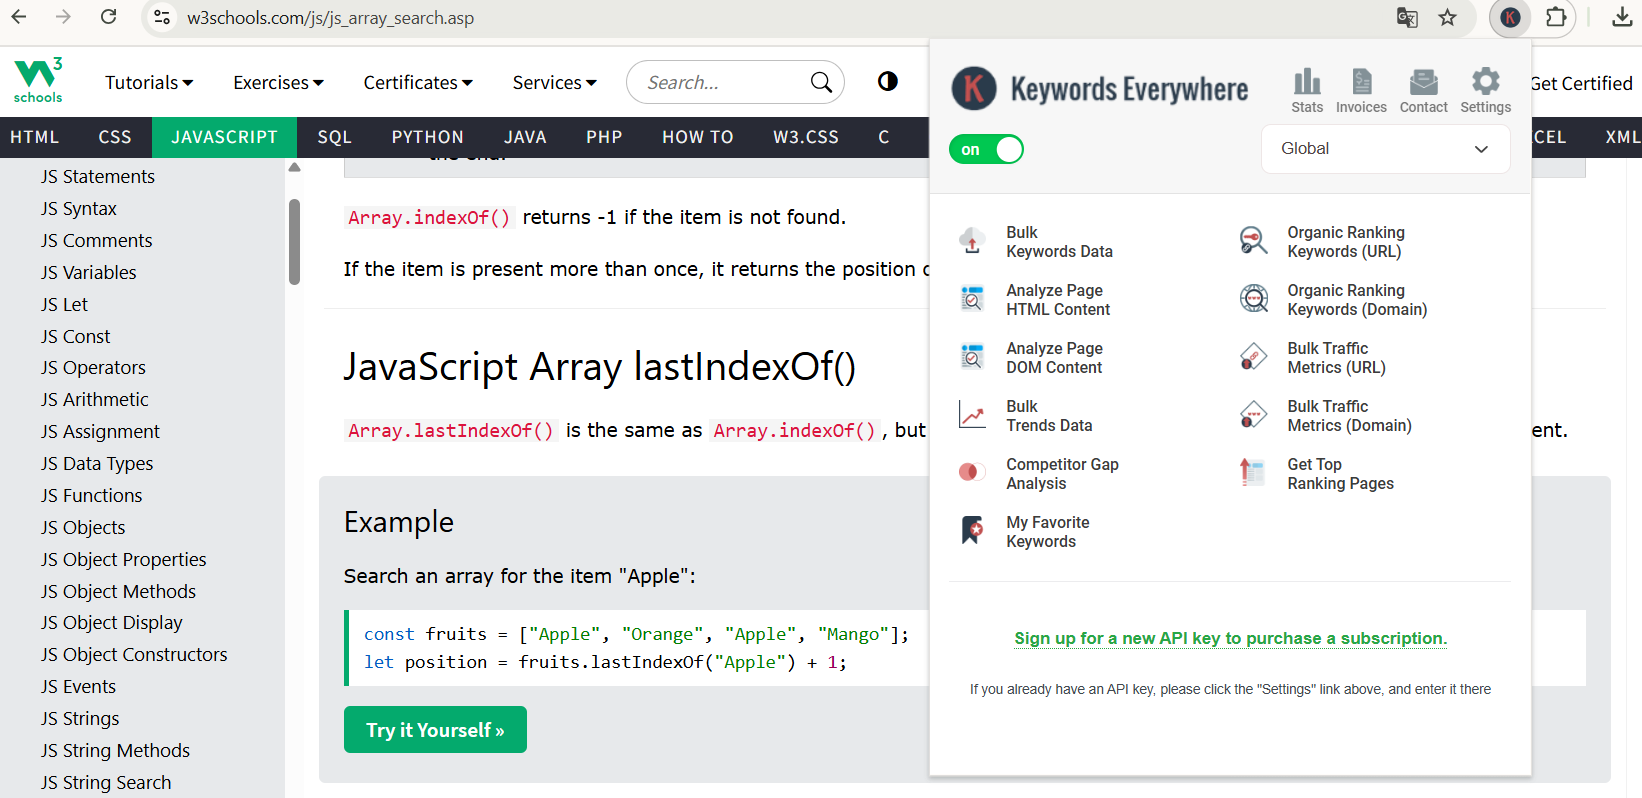
\includegraphics[width=0.9\textwidth]{soluzioni-esistenti/Keywords-Everywhere/keywords_everywhere.png} 
    \caption{Keywords Everywhere}
\end{figure}

\section{SEO Minion}

\subsection{Funzionalità}
\par SEO Minion è un tool specializzato nell’analisi SEO fornito da Keywords Everywhere. Tra le attività svolte da SEO Minion, le più significative sono:
\begin{itemize}
    \item \textbf{Analisi SEO On-page}: identifica problemi nella struttura delle pagine web;
    \item \textbf{Controllo link}: evidenzia i link interni ed esterni presenti all’interno della pagina;
    \item \textbf{Controllo "broken link"}: identifica eventuali "broken link" e li classifica in base ai codici di stato;
    \item \textbf{Preview e utility SERP}: visualizza un'anteprima del sito su un risultato di ricerca reale e scarica dati dalla SERP (Search Engine Results Page);
    \item \textbf{SERP multi-località}: controlla il posizionamento del sito in base a diverse combinazioni di localizzazione/lingua;
    \item \textbf{HTML vs DOM}: analizza le differenze tra il codice sorgente e il DOM renderizzato.
\end{itemize}

\begin{figure}[H] 
    \centering 
    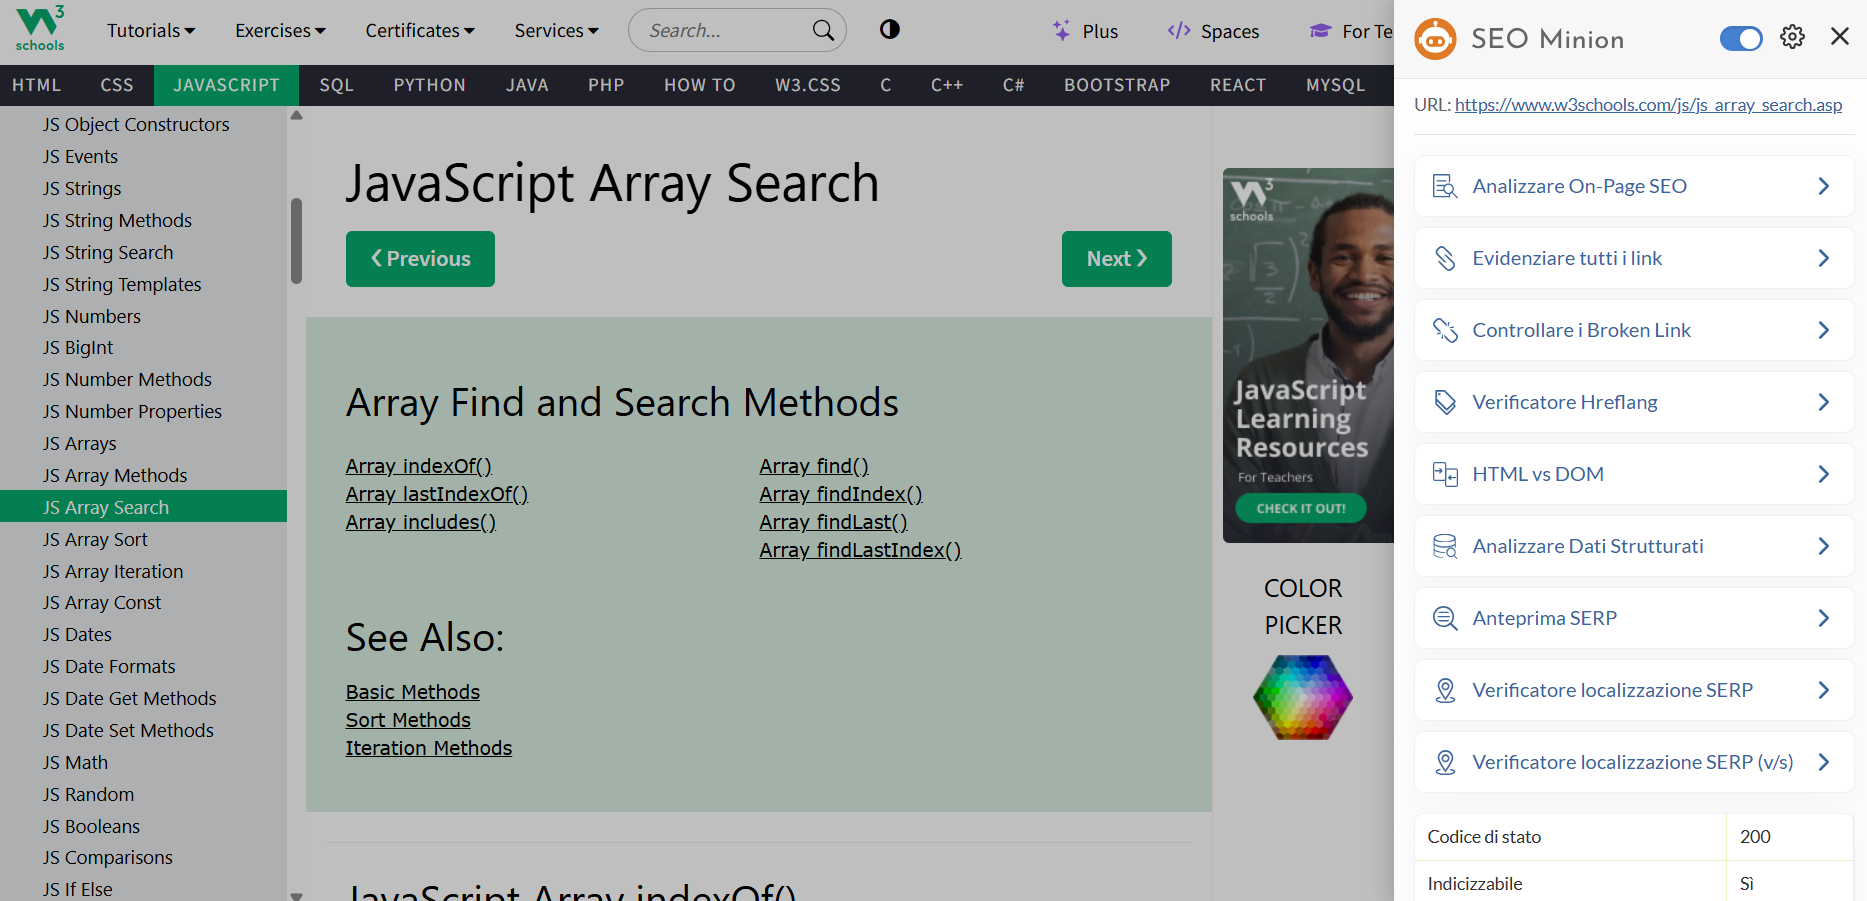
\includegraphics[width=0.9\textwidth]{soluzioni-esistenti/SEO-Minion/seo_minion_sidebar.png} 
    \caption{SEO Minion - sidebar}
\end{figure}

\subsection{Vantaggi}
\par SEO Minion è disponibile come estensione o add-on per Google Chrome, Firefox e Microsoft Edge. Le funzionalità di analisi SEO sono integrate in un'unica piattaforma.

\subsection{Svantaggi}
\par SEO Minion è disponibile solo per i clienti del piano Silver o superiore di Keywords Everywhere.

\begin{figure}[H]
    \centering 
    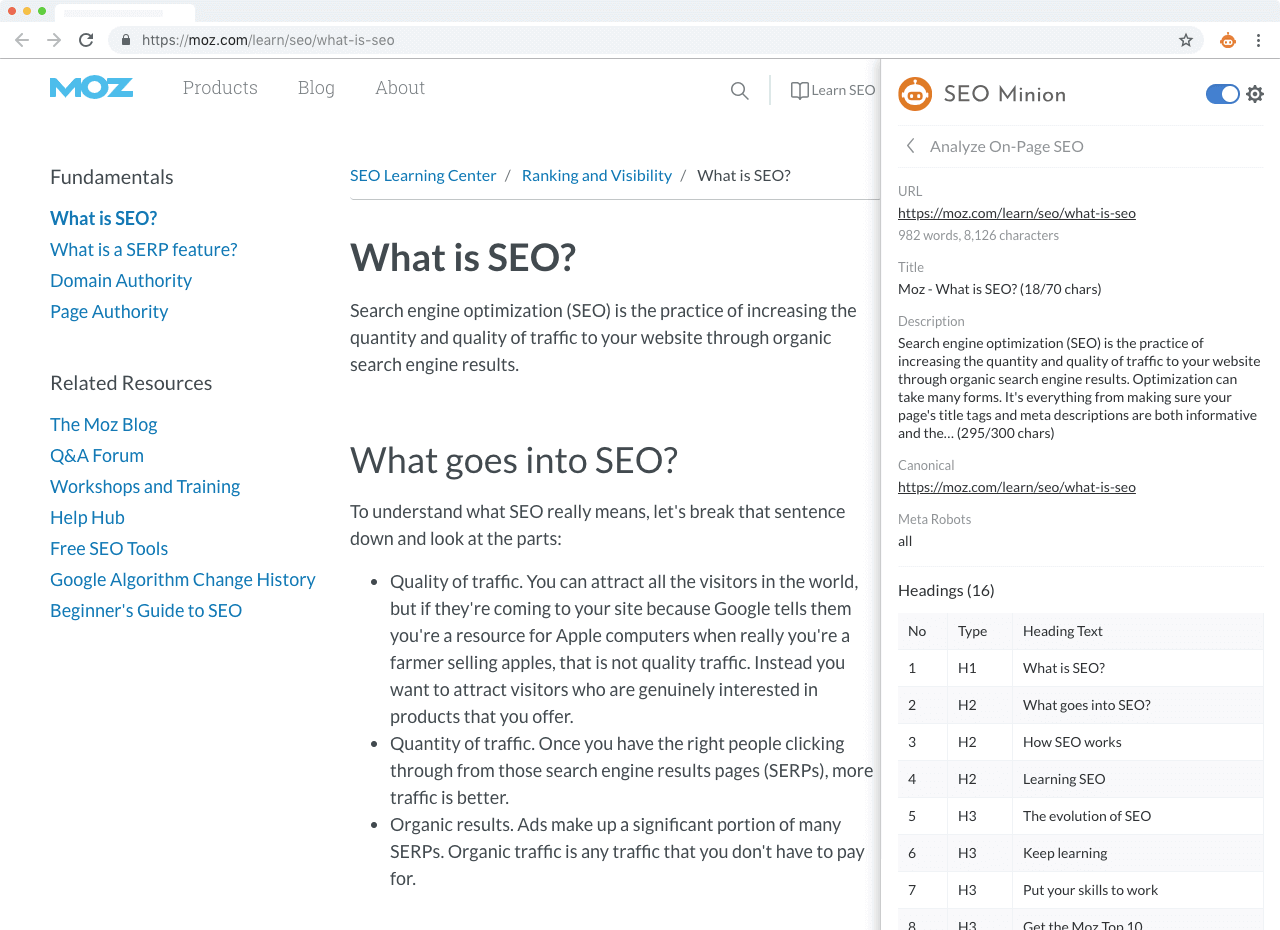
\includegraphics[width=0.8\columnwidth]{soluzioni-esistenti/SEO-Minion/seo_minion_on_page_analysis.png} 
    \caption{SEO Minion - Analisi On-Page}
\end{figure}

\section{SEO Checker}

\subsection{Funzionalità}
\par SEO Checker è uno strumento dell’ecosistema Keywords Everywhere, all’interno del quale troviamo anche il già citato SEO Minion. Mentre quest’ultimo è stato concepito per l’analisi single-page, SEO Checker nasce per superarne i limiti: permette infatti di analizzare siti con migliaia di pagine e integra controlli su velocità e sicurezza.

\begin{figure}[H]
    \centering 
    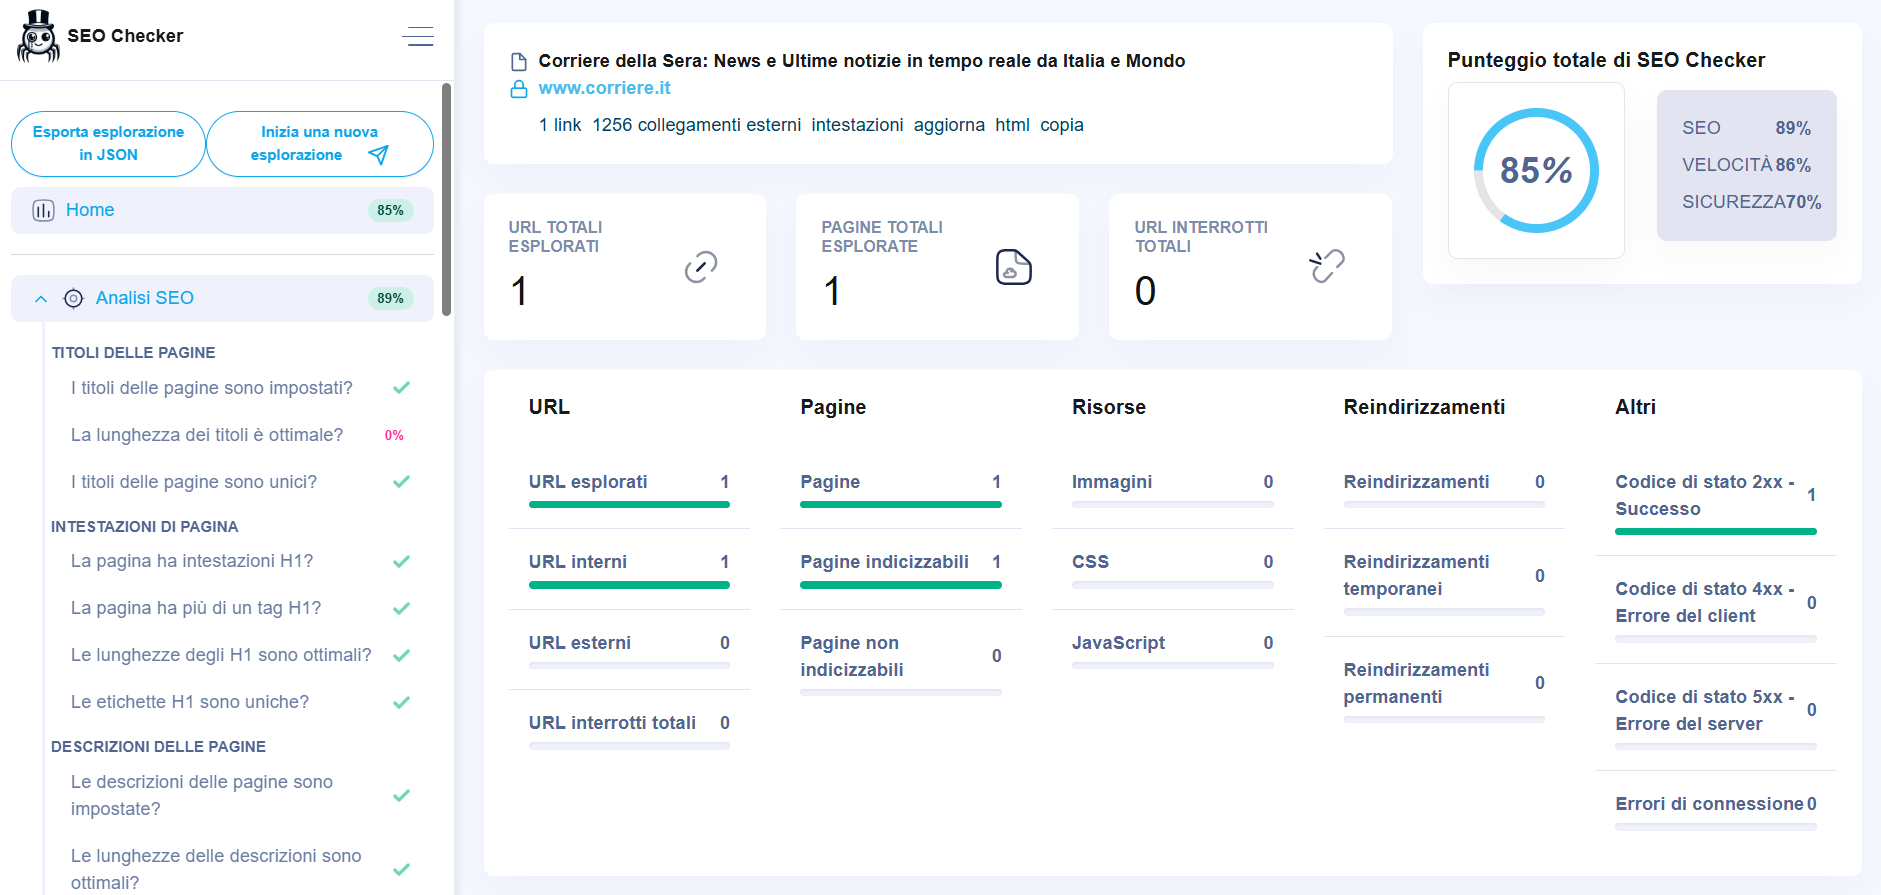
\includegraphics[width=0.8\columnwidth]{soluzioni-esistenti/SEO-Checker/seo_checker_analysis.png} 
    \caption{SEO Checker - Analisi SEO del Corriere della Sera}
\end{figure}

\subsection{Vantaggi}
\par Così come SEO Minion, anche SEO Checker è disponibile come estensione o add-on per Google Chrome, Firefox e Microsoft Edge. Le funzionalità sono integrate in un'unica piattaforma. A differenza di SEO Minion, SEO Checker è disponibile gratuitamente.

\subsection{Svantaggi}
\par SEO Checker fornisce un'analisi dettagliata della SEO on-page, ma risulta carente per quanto riguarda le funzionalità di ricerca e analisi delle parole chiave.

\section{Yoast SEO (plugin per CMS)}

\subsection{Funzionalità}
\par Yoast SEO è un plugin per CMS che semplifica il processo di ottimizzazione SEO. Fornisce feedback in tempo reale per migliorare il posizionamento sui motori di ricerca. La versione del plugin per WordPress consente di ottimizzare le parole chiave (note anche come keyphrase) attraverso un’analisi della densità, della distribuzione e di altri fattori SEO on-page. Con la versione a pagamento, l’utente può anche scegliere delle keyphrase correlate (argomenti collegati o parole chiave secondarie) da valutare distintamente. Inoltre, l’integrazione con Semrush fornisce suggerimenti di keyphrase correlate basati sui volumi di ricerca, sull’intento e sulla keyword difficulty. Naturalmente, i controlli sono meno restrittivi rispetto alla parola chiave principale. Per evitare di dover ripetere meccanicamente la stessa keyphrase, la versione Premium permette anche di aggiungere uno o più sinonimi, che Yoast interpreta allo stesso modo senza penalizzare il punteggio.

\begin{figure}[H]
    \centering 
    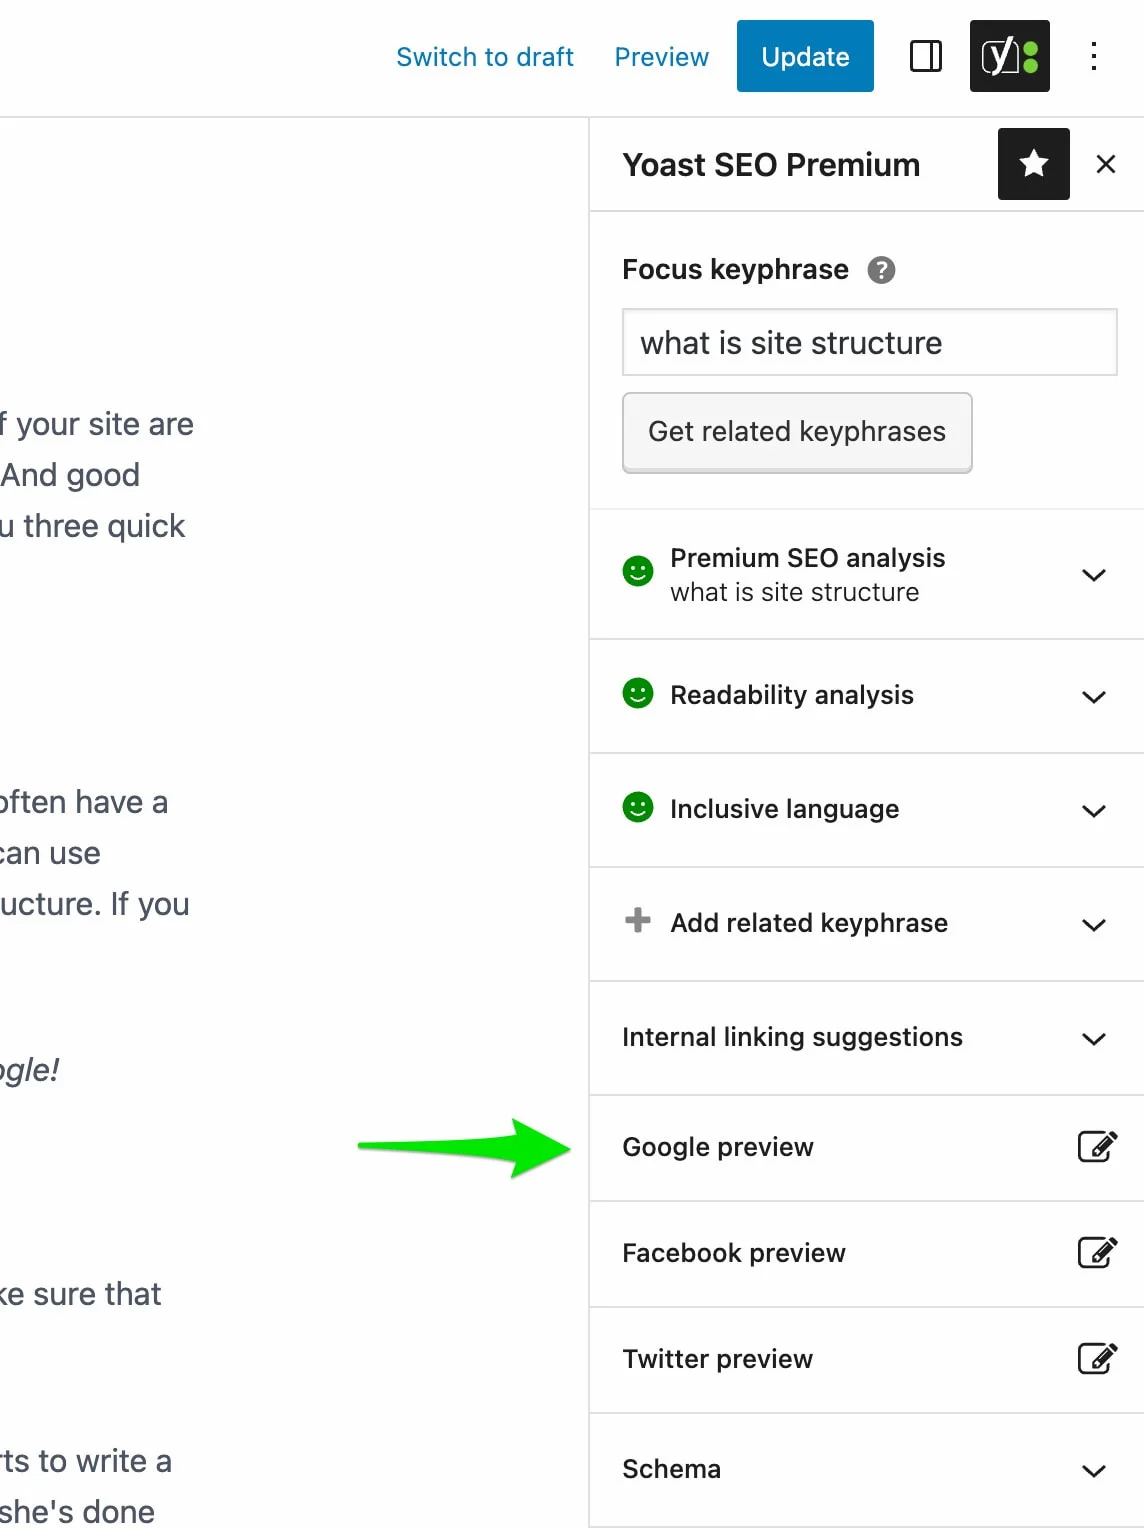
\includegraphics[width=0.4\columnwidth]{soluzioni-esistenti/Yoast-SEO/yoast_seo_sidebar.png} 
    \caption{Yoast SEO - sidebar}
\end{figure}

\subsection{Vantaggi}
\par Yoast SEO è disponibile in versione gratuita per WordPress, seppur con alcune limitazioni, e può essere integrato con altri strumenti SEO come Semrush e Wincher. Il plugin viene aggiornato regolarmente per rimanere allineato agli algoritmi dei motori di ricerca e alle best practice SEO.

\subsection{Svantaggi}
\par Yoast SEO è limitato a CMS come WordPress e Shopify. Alcune funzionalità, tra cui l’inserimento di parole chiave correlate e sinonimi, o l'integrazione con Semrush, richiedono la sottoscrizione di un abbonamento a pagamento.

\begin{figure}[H]
    \centering 
    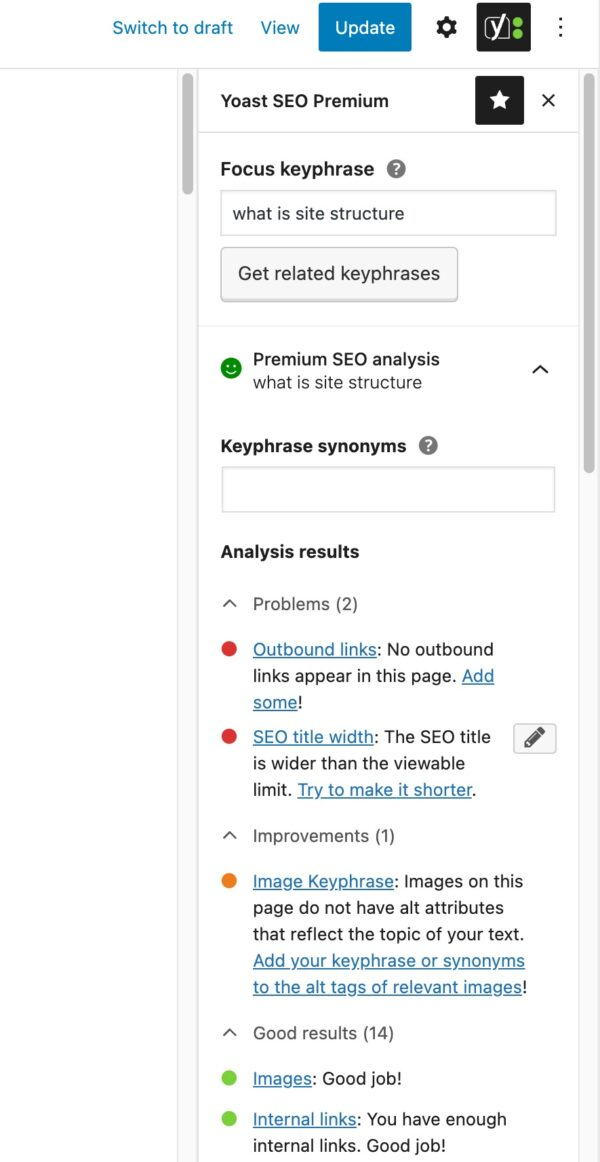
\includegraphics[width=0.4\columnwidth]{soluzioni-esistenti/Yoast-SEO/yoast_seo_premium.png} 
    \caption{Yoast SEO Premium - Analisi SEO}
\end{figure}

\section{Keyword Density Analyzer}

\subsection{Funzionalità}
\par 

\section{Detailed SEO Extension}

\subsection{Funzionalità}
\par Detailed SEO Extension è un’estensione per Google Chrome e Firefox che consente di analizzare, con un solo clic, qualsiasi sito web. L’estensione estrae e analizza i seguenti elementi:
\begin{itemize}
    \item Titolo, meta description, URL, tag canonical, tag "robots", meta tag keywords, numero di parole e lingua;
    \item Gerarchia degli heading (da H1 a H6): l'estensione regola l'indentazione e la dimensione del font in base al livello, facilitando l'analisi visiva della struttura;
    \item Link (unici, interni o esterni, completi o incompleti);
    \item Immagini (complete o prive di attributi);
    \item Schema e Hreflang;
    \item Open Graph.
\end{itemize}
\par Inoltre, l'estensione genera automaticamente i link per analizzare la stessa pagina web su altre piattaforme, tra cui Ahrefs, Majestic, Moz, Semrush e SimilarWeb.

\begin{figure}[H]
    \centering 
    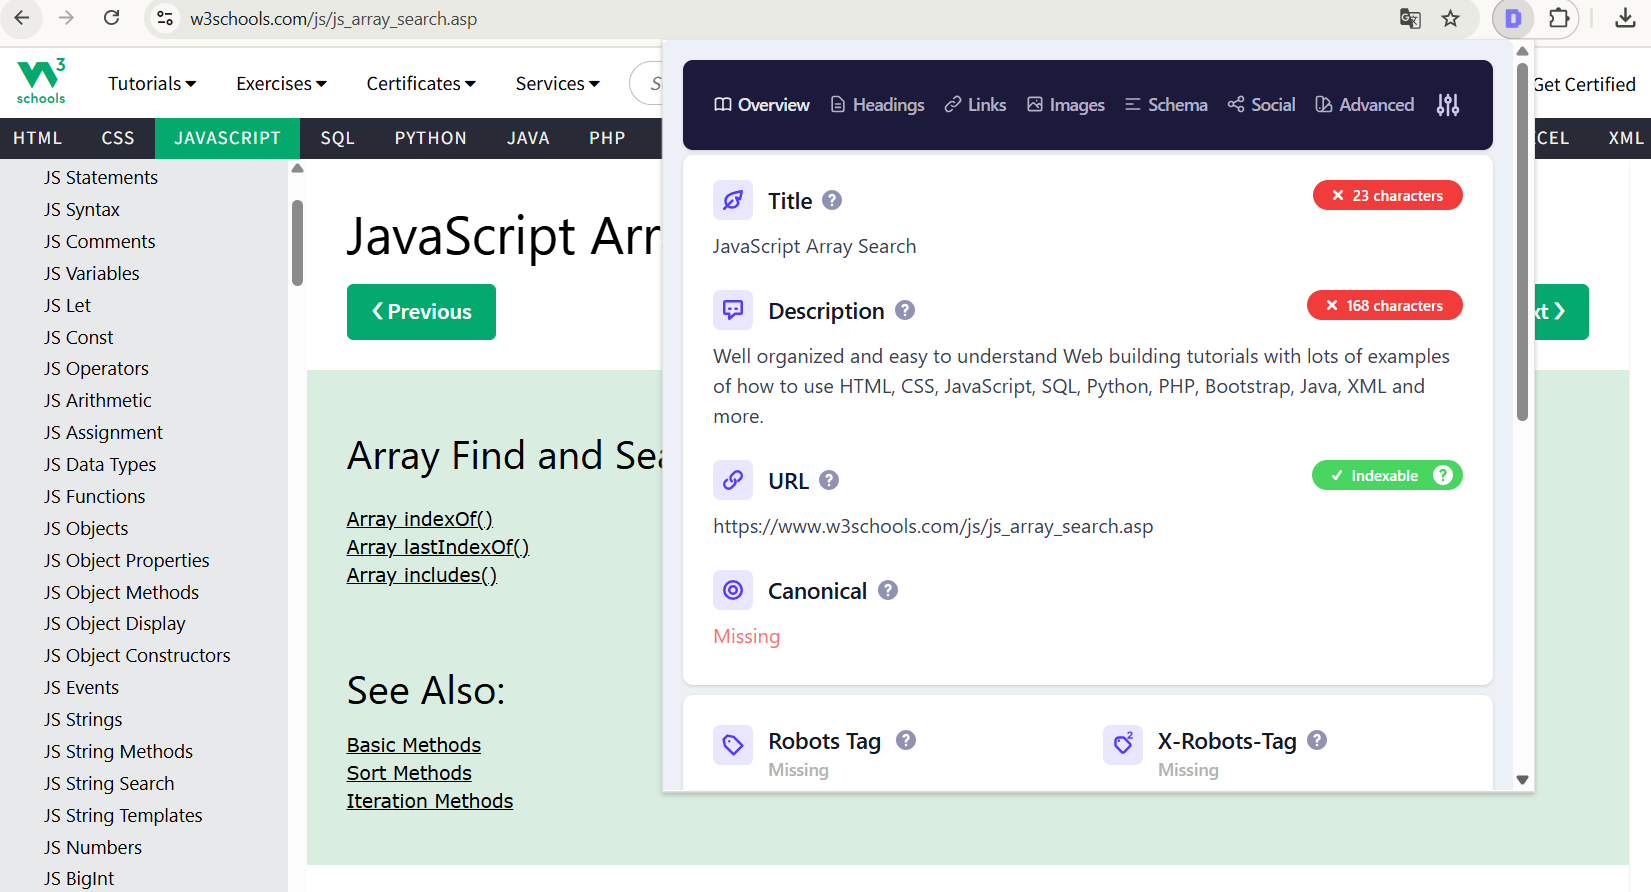
\includegraphics[width=0.8\columnwidth]{soluzioni-esistenti/Detailed-SEO-Extension/detailed_seo_extension.png} 
    \caption{Detailed SEO Extension}
\end{figure}

\subsection{Vantaggi}
\par Essendo gratuita e compatibile con localhost, l'estensione si presta perfettamente all'uso durante la fase di sviluppo.

\subsection{Svantaggi}
\par L'estensione si apre come pop-up, il che può rendere meno agevole l'interazione con la pagina corrente. Per quanto riguarda l'analisi delle parole chiave, lo strumento si limita a estrarre ed elencare quelle presenti nel meta tag `keywords`.

\begin{figure}[H]
    \centering 
    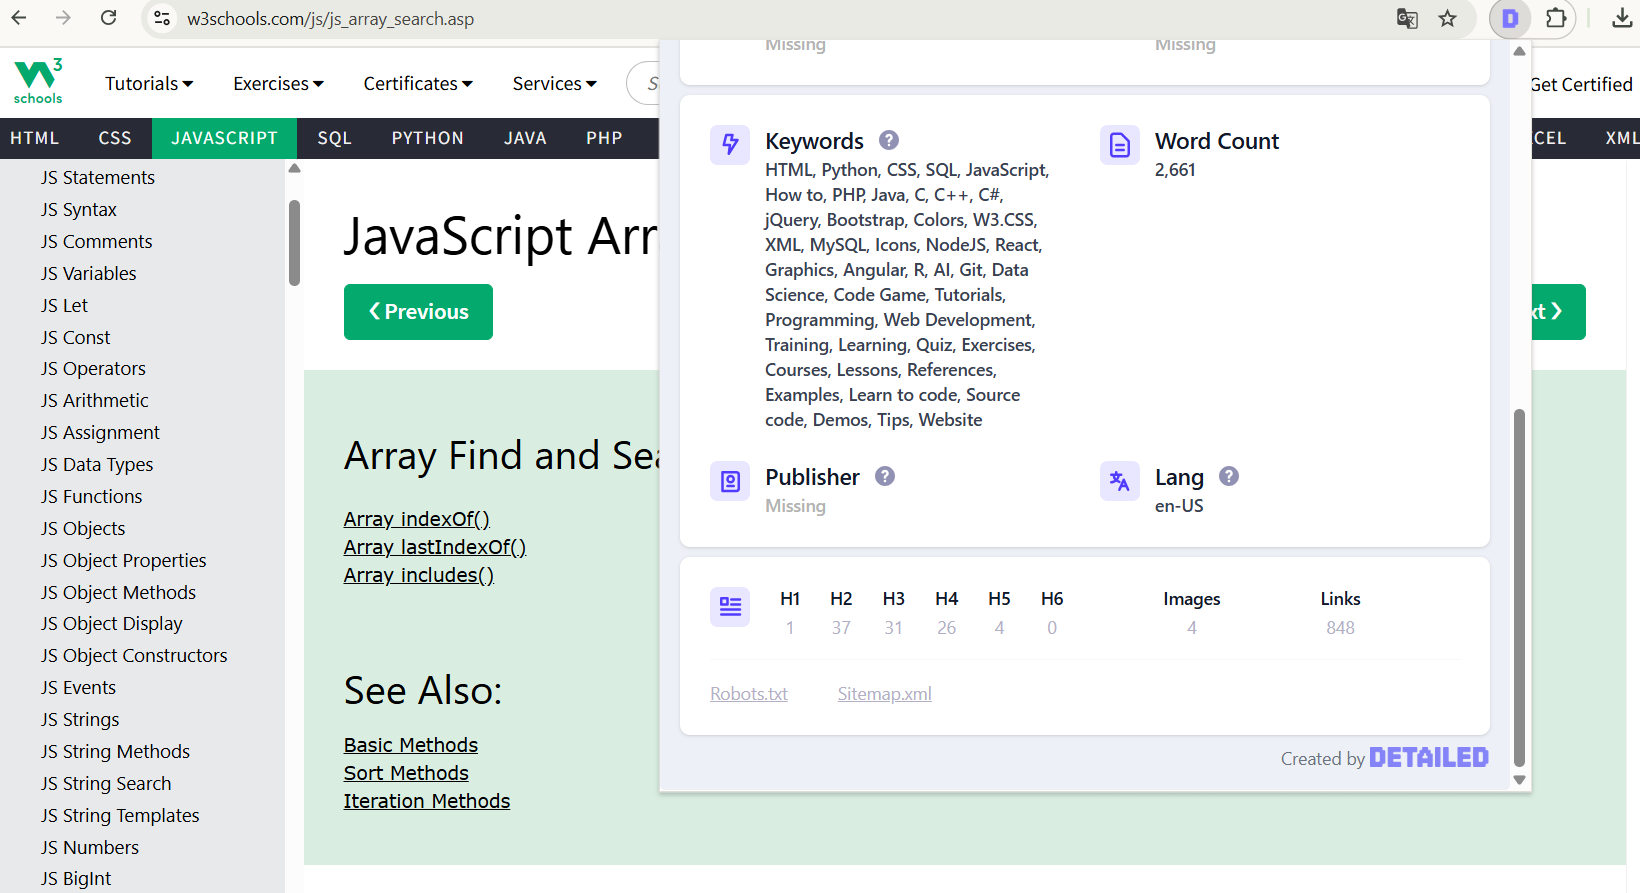
\includegraphics[width=0.8\columnwidth]{soluzioni-esistenti/Detailed-SEO-Extension/detailed_seo_analysis.png} 
    \caption{Detailed SEO Extension - Analisi SEO}
\end{figure}

\section{Checkbot}

\subsection{Funzionalità}
\par Checkbot è un'estensione per browser che esegue analisi SEO, test di velocità e di sicurezza su centinaia di pagine contemporaneamente.

\subsection{Vantaggi}
\par Checkbot fornisce un'analisi SEO on-page completa.

\subsection{Svantaggi}
\par Per accedere a funzionalità essenziali per lo sviluppo, come l'analisi su localhost, è necessario un abbonamento a pagamento. I test vengono eseguiti sulla piattaforma web di Checkbot e non includono l'analisi delle parole chiave.

\begin{figure}[H]
    \centering 
    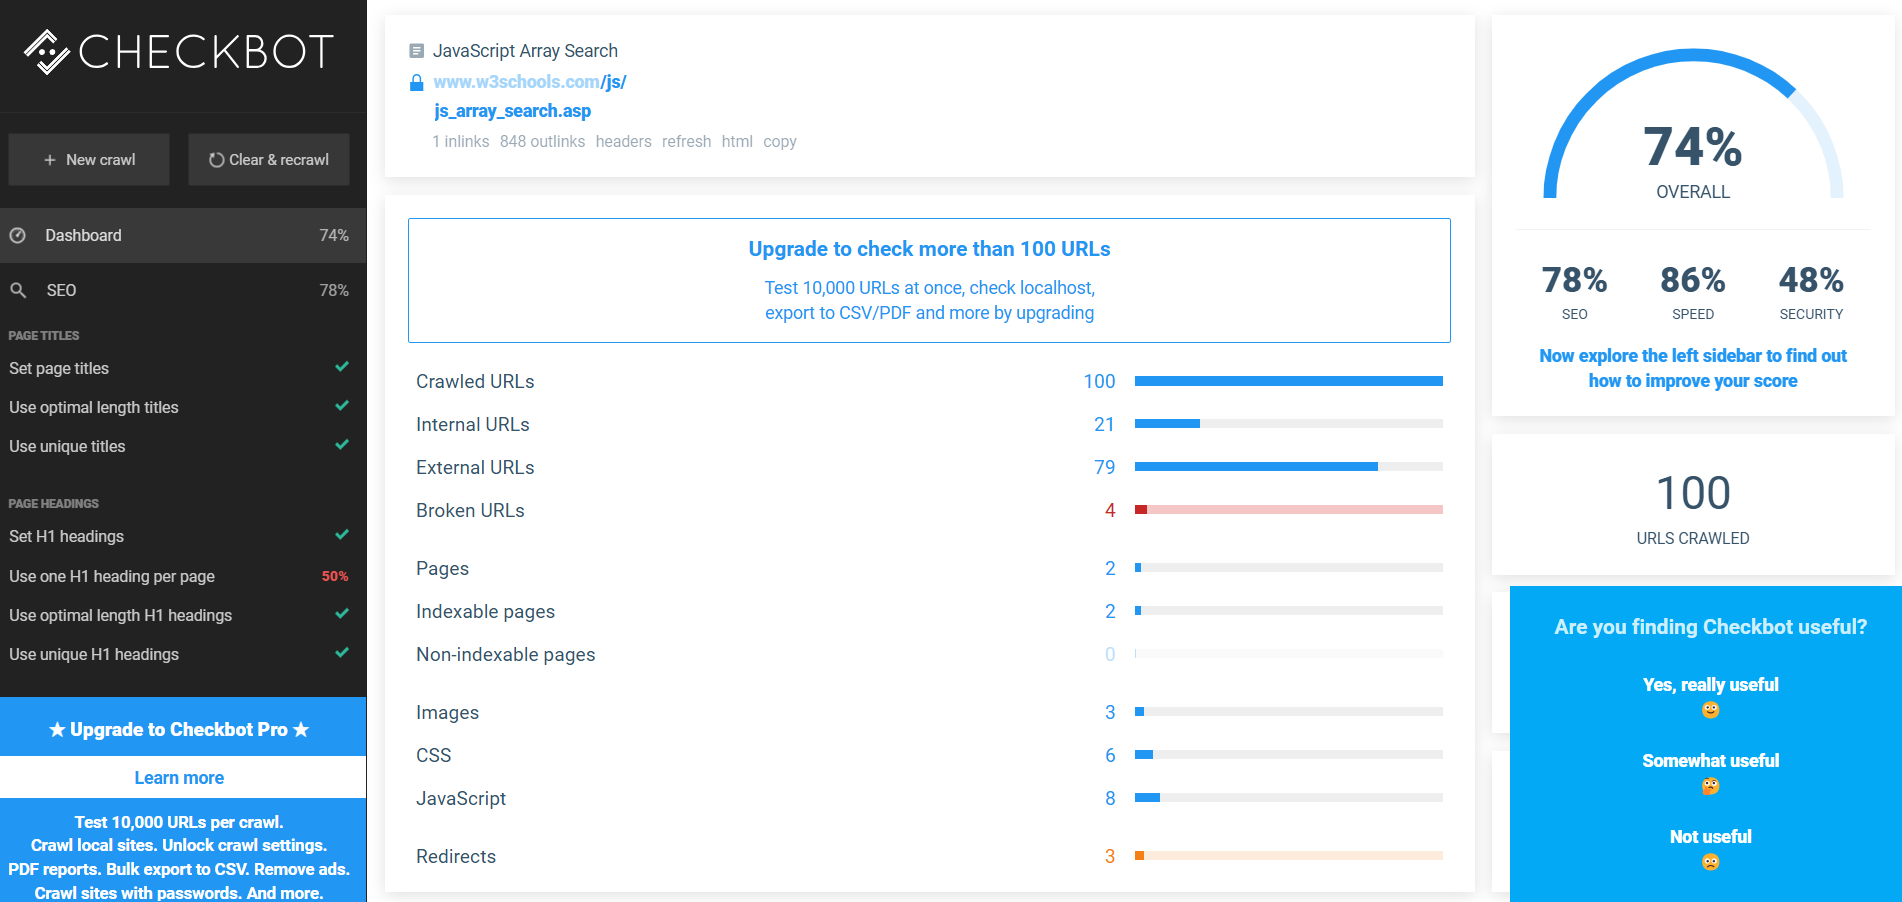
\includegraphics[width=0.8\columnwidth]{soluzioni-esistenti/Checkbot/checkbot.png} 
    \caption{Checkbot}
\end{figure}

\section{Serpstat}

\subsection{Funzionalità}
\par Checkbot è un'estensione per browser che esegue analisi SEO, test di velocità e di sicurezza su centinaia di pagine contemporaneamente.

\section{Sitebulb}

\subsection{Funzionalità}
\par Checkbot è un'estensione per browser che esegue analisi SEO, test di velocità e di sicurezza su centinaia di pagine contemporaneamente.

\section{Screaming Frog SEO}

\subsection{Funzionalità}
\par Checkbot è un'estensione per browser che esegue analisi SEO, test di velocità e di sicurezza su centinaia di pagine contemporaneamente.

\section{Wincher}

\subsection{Funzionalità}
\par Checkbot è un'estensione per browser che esegue analisi SEO, test di velocità e di sicurezza su centinaia di pagine contemporaneamente.

\section{Majestic}

\subsection{Funzionalità}
\par Checkbot è un'estensione per browser che esegue analisi SEO, test di velocità e di sicurezza su centinaia di pagine contemporaneamente.

\section{Similarweb}

\subsection{Funzionalità}
\par Checkbot è un'estensione per browser che esegue analisi SEO, test di velocità e di sicurezza su centinaia di pagine contemporaneamente.

\section{Ahrefs SEO Toolbar}

\subsection{Funzionalità}
\par Ahrefs SEO Toolbar è un'estensione gratuita per browser che esegue un'analisi SEO completa e dettagliata.

\subsection{Vantaggi}
\par L'estensione funziona su localhost e fornisce suggerimenti SEO direttamente nei risultati di ricerca.

\subsection{Svantaggi}
\par Per accedere alle metriche avanzate di Ahrefs, è necessario un abbonamento a pagamento. Inoltre, l'estensione si apre solo come pop-up, il che può interferire con la navigazione.

\begin{figure}[H]
    \centering 
    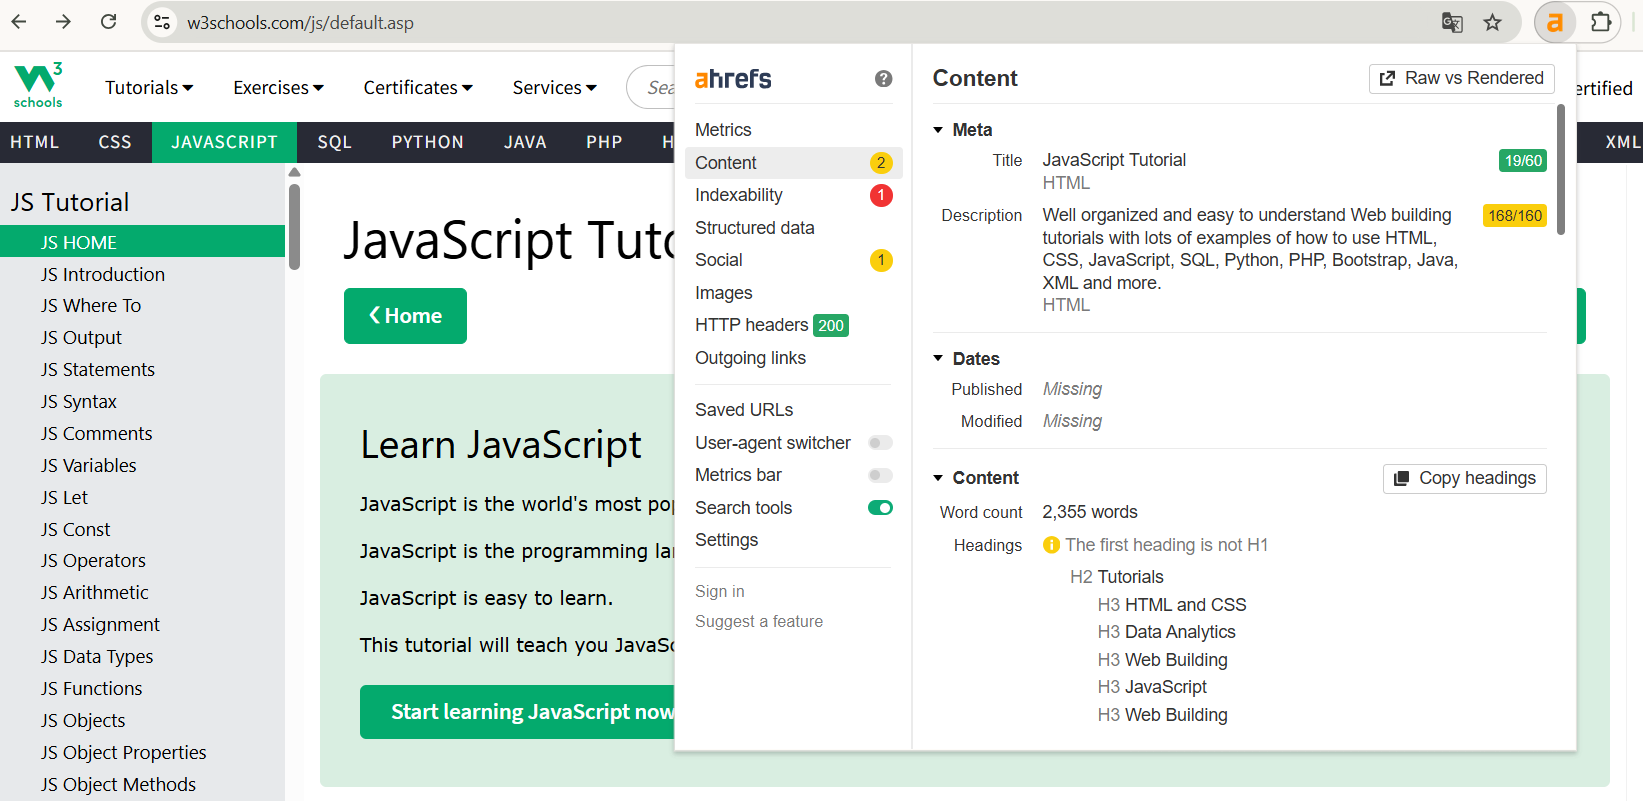
\includegraphics[width=0.8\columnwidth]{soluzioni-esistenti/Ahrefs/ahrefs.png} 
    \caption{Ahrefs SEO Toolbar}
\end{figure}

\section{Ubersuggest}

\subsection{Funzionalità}
\par Ubersuggest è uno strumento SEO disponibile sia come piattaforma web esterna che come estensione gratuita per Chrome. Fornisce analisi del traffico organico e a pagamento, suggerimenti di parole chiave, analisi dei backlink e dei competitor.

\subsection{Vantaggi}
\par L'estensione è progettata come barra laterale, facilitando l'interazione con la pagina corrente.

\subsection{Svantaggi}
\par Nella versione gratuita, le funzionalità sono limitate a 40 richieste al giorno. Inoltre, l'accesso a dati e funzioni avanzate richiede l'upgrade a un piano a pagamento.

\section{Keyword Surfer}

\subsection{Funzionalità}
\par Keyword Surfer è un’estensione per Chrome che mostra volumi di ricerca e suggerimenti di parole chiave direttamente nei risultati di ricerca. Fornisce anche informazioni sulle pagine dei competitor, come il traffico stimato e il numero esatto di occorrenze di una parola chiave.

\subsection{Vantaggi}
\par La ricerca e l'analisi delle parole chiave sono completamente gratuite.

\subsection{Svantaggi}
\par Rispetto ad altre piattaforme SEO, Keyword Surfer offre funzionalità più limitate.